\documentclass[titlepage,a4paper]{jsarticle}
\usepackage{../../../sty/import}% 各種パッケージインポート
\usepackage{../../../sty/title}% タイトルページの変更
\renewcommand{\thesection}{問\arabic{section}}
% 右上側に名前,学籍番号,提出日の記述が必要なので,急遽付け足し
\usepackage{fancyhdr}
\pagestyle{fancy}
  \lhead{情報社会と著作権最終課題}
  \rhead{
    \begin{tabular}[t]{>{\bfseries}l@{\hspace{0.5\zw}:\hspace{0.5\zw}}l}
      氏名   & 本間三暉\\
      学籍番号 & 24336488\\
      提出日  & \today
    \end{tabular}
  }
%% タイトルページの変数
% レポートタイトル
\title{情報と著作権最終課題}
% 提出日
\expdate{\today}
% 科目名
\subject{情報社会と著作権}
% 分野
\class{情報経営システム工学分野}
% 学年
\grade{B3}
% 学籍番号
\mynumber{24336488}
% 記述者
\author{本間三暉}

\begin{document}
% titleページ作成
\maketitle
\section{「情報」の概念および性質について、現代のデジタル化、ネットワーク化との関連に触れつつ説明せよ。}
情報の性質として大きく分けて3つが挙げられる.

1つ目が独占に向かないという情報の非競合性である.
これは一人で使おうが1000人で使おうが減らないという性質である.

2つ目は占有管理が難しいという情報の非排除性である.
これは優先物ならば管理が良い腕使われたらすぐに分かるが「情報」は無体物であり管理が困難であるというものである.

3つ目は拡散しやすいという情報の拡散性である.
これは一度知られた情報が他に広がるのを防ぐのは困難であるというものである.

特に情報の拡散性に関して,近年の急速なデジタル化・ネットワーク化によりこの性質が急激に顕在化している.

\section{近年、違法コピーされた漫画などのコンテンツをインターネット経由で閲覧できるウェブサイトの存在が社会問題となっている。
  上記のようにウェブサイト運営者が違法コピーされたコンテンツをインターネット経由で提供できるようにする行為は、著作権法におけるどのような権利(〇〇権といわれる支分権)を侵害する行為であるか説明せよ。
  また、このようなウェブサイトを利用するユーザの行為が刑事罰の対象になる場合とならない場合について説明せよ。}
違法にコピーされた漫画などのコンテンツをインターネット上で提供するウェブサイトの運営者は,著作権法における「公衆送信権」を侵害している.
公衆送信権とは,著作物を公衆に対して送信する権利であり,インターネットを通じてコンテンツを配信する行為がこれに該当する.
したがって,著作権者の許可なく違法コピーされたコンテンツをウェブサイトで提供することは公衆送信権の侵害となる.

次に,このようなウェブサイトを利用するユーザの行為が刑事罰の対象となる場合とならない場合について説明する.
一般的に,違法にアップロードされたコンテンツをダウンロードする行為は著作権法に違反する可能性がある.
特に,音楽や映像などの違法コンテンツをダウンロードする行為は刑事罰の対象となる.
一方で,違法にアップロードされたコンテンツをストリーミング再生するだけの場合,現行の著作権法では刑事罰の対象とはならない.
しかし,違法コンテンツの視聴行為が著作権法に違反する可能性があるため注意が必要である.\cite{task2}

以上のことから,違法コピーされたコンテンツを提供するウェブサイトの運営者は公衆送信権を侵害しており,
その利用者も違法コンテンツのダウンロード行為によって刑事罰の対象となる可能性があるため正規の方法でコンテンツを利用することが重要である.
\section{ }
注意:他人の写真(ネット検索で拾った写真を含む)の利用が発覚した場合には期末レポート全体をゼロ点評価とする。
結果、単位も取得できなくなるので絶対に他人の写真は使用しないこと。
\subsection{著作物の定義について示し、かつ、その定義に含まれる4つの要件についてそれぞれ簡単に説明せよ。}
著作物とは,思想または感情を創作的に表現したものであり,文芸,学術,美術,音楽の範囲に属するものを指す.\cite{task3_1}

著作物として認められるためには,次の4つの要件を満たす必要がある.

まず,著作物には「思想または感情」が含まれていなければならない.
これは,作者の内面的な考えや感情が表現されていることを意味し,単なる事実やデータの羅列ではこの要件を満たさない.

次に,著作物には「創作的」であることが求められる.
他人の作品をそのまま模倣したものやありふれた表現だけで構成されているものには創作性が認められず,著作物とはみなされない.

また,著作物は「表現されたもの」である必要がある.
アイデアや概念だけではなく,それが具体的な形に落とし込まれていることが重要である.

最後に,その作品が「文芸,学術,美術,音楽」のいずれかの範囲に属していることが必要である.
これらの文化的・芸術的分野に該当しない場合,著作物として保護されない.

以上の4つの要件をすべて満たした場合,作品は著作物として認められ,著作権法による保護の対象となる.

\newpage
\subsection{写真の著作物の創作性に関し、各自、自分で撮影した写真をレポート中に貼り付けて提示した上でその写真には著作権法上の観点でいかなる点に著作者であるあなたの個性が現れており創作性があるのかを説明せよ。
  なお、例えば構図について説明する場合であれば、単に「構図に創作性がある」などとするのではなく、写真の内容に基づいて「構図について〇〇〇〇という点で創作性がある」というように具体的に説明すること。}
私が今回撮影した写真を図\ref{food}に示す.

\begin{figure}[H]
  \centering
  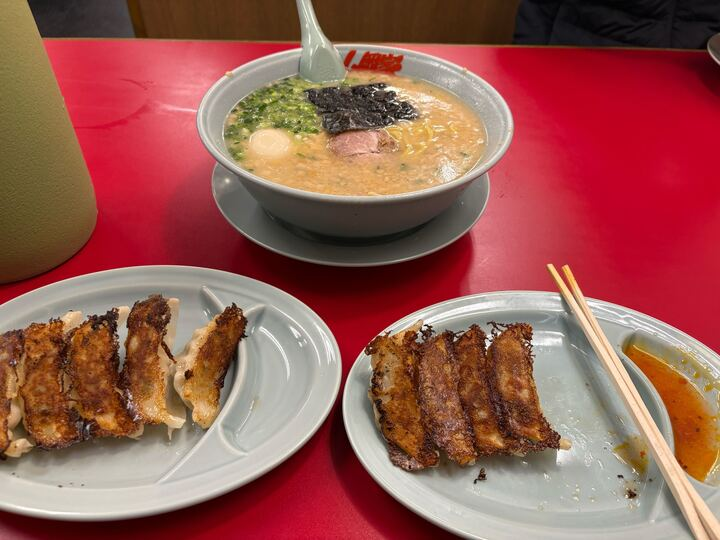
\includegraphics[width=0.8\textwidth]{img/img_task3_2.png}
  \caption{山岡家で撮影したプレミアム塩豚骨と餃子}
  \label{food}
\end{figure}

この写真には,プレミアム塩とんこつラーメンと餃子が2つ写っている.
お店で提供される食べ物の写真を撮ろうと思ったら自分でお金を出して頼まなければならないが,
プレミアム塩豚骨と餃子を2つ頼み食べきるような人は私を除いてそう多くない.
よってそもそもこの状況の再現性が低い.またたくさん食べたいという感情が伝わってくる.

また,この画像では餃子のお皿にたれが入れられており,右のお皿の餃子が左のお皿の餃子が減っていることや割り箸にたれがついていることから,
餃子を食べたあとに写真を取ったことがわかる.
美味しい食べ物の写真を撮る際食べかけの様子を撮ることは少なく,届いた状態の写真を撮ることが多い.
加えて,山岡家という特別餃子が美味しいと有名な店でないお店で二皿も頼む人はもっと少ない.
そのため,あえてそのような状態を撮っている写真は創作性があると考えられる.

次に,普通の人が頼むには多い量を頼んでいることからお腹が空いているという気持ちを表現していると言える.

最後に,この著作物は写真であり,写真は写真は絵画や彫刻と同様に,感情や思想を視覚的に表現し,
観る者に深い感動や思索を促す力を持つため広く芸術の一形態として認識されている.

\subsection{上記の写真について他人により勝手にトリミングされる等の改変がなされたとする。
  この改変が自分の思い入れのある部分を台無しにするもので許せないと感じた場合に、あなたはその他人に対してどのような権利を主張することができるかを説明せよ。}
自ら撮影した写真が他人によって無断でトリミングされ,思い入れのある部分が損なわれた場合,著作者として「同一性保持権」を主張することができる.
同一性保持権とは,著作物およびその題号について,著作者の意に反して変更,切除,その他の改変を禁止できる権利である.
この権利は,著作者の人格的利益を保護するために設けられており,無断でのトリミングや改変が著作者の意図に反する場合,同一性保持権の侵害となる.\cite{task3_2}

例えば,写真の上下または左右を一部切除して掲載した事例において,裁判所は「上下又は左右の一部が切除されたことにより各写真の本来の構図が明らかに変更されており,
これによって著作者の制作意図に沿わないものとなっている」と判断し,同一性保持権の侵害を認めた判例がある.\cite{task3_3}

したがって,無断でのトリミングが著作者の意図や感情を損なうものである場合,同一性保持権の侵害として,改変の中止や損害賠償を求めることが可能である.

\section{ }
\subsection{著作物の「複製」の定義と「翻案」の定義をそれぞれ示し、あわせて「依拠性」及び「同一性」についても説明せよ。}
著作物の「複製」とは,著作物を有形的に再製することを指し,印刷,写真,複写,録音,録画などの方法で行われる.
一方,「翻案」とは,既存の著作物に依拠し,その表現上の本質的な特徴を維持しつつ,具体的表現に修正,増減,変更などを加えて,
新たに思想または感情を創作的に表現することをいう.
これにより,既存の著作物の表現上の本質的な特徴を直接感得できる別の著作物が創作される.

「依拠性」とは,ある著作物が既存の著作物に基づいて作られていることを指す.
つまり,新たな著作物が既存の著作物を参考にして創作された場合,依拠性が認められる.
依拠性は,著作権侵害を判断する際の重要な要素であり,侵害を主張する側が,既存の著作物へのアクセス可能性や類似性を示すことで立証される.

「同一性」とは,著作物の内容や形式が,元の著作物とどれだけ一致しているかを示す概念である.
複製の場合,元の著作物と実質的に同一であることが求められるが,多少の修正や増減があっても,著作物の同一性を損なわない限り,複製とみなされる.
翻案の場合は,元の著作物の本質的な特徴が残存しているか(類似性)が問題となり,新たな創作的表現が加えられていても,元の著作物の本質的特徴が直接感得できる場合,翻案とされる.

以上のように,複製と翻案は,既存の著作物に依拠して新たな作品を作成する行為であり,依拠性と同一性は,これらの行為が著作権侵害に該当するかどうかを判断する際の重要な要素である.\cite{task4}

\subsection{図\ref{miffy}に提示する2つのキャラクターのうち、右側の「キャシー」は左側の「ミッフィー」の複製ないし翻案に当たるかどうか、自分の考えを論述せよ。
  ただし、「キャシー」の創作時点において「ミッフィー」はすでに公開されており、その事実を「キャシー」のデザイナーは知っていたものとする。}
\begin{figure}[H]
  \centering
  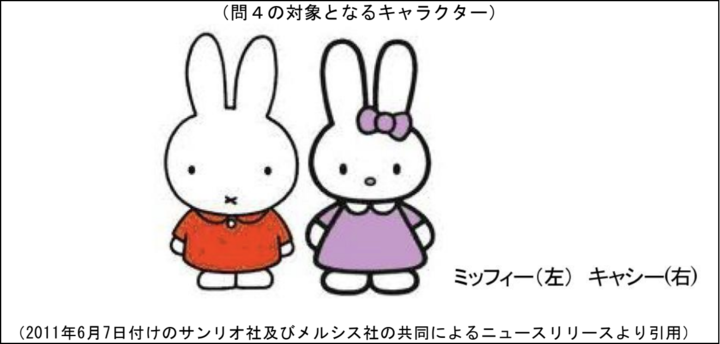
\includegraphics[width=5cm]{img/img_task4.png}
  \caption{問4の対象となるキャラクター}
  \label{miffy}
\end{figure}
% 注意:結論はどちらでもよい。論述の内容を評価する。法学部生のような厳格な法律論は求めていない。
% 自分なりの考えが根拠とともに示されていればよい。ネットで得た情報を参考にするのは構わないがコピペの疑われる回答はゼロ点評価とする。
図\ref{miffy}を見ると確かにこの2つのキャラクターは似ているという感想を持つ.
しかし,細かく見てみると,口や顔の大きさ,リボンの有無など異なる点は多い.
また,うさぎを題材に擬人化すると考えたときに,長い耳と二頭身で直立していて服を着ているという大きな特徴は著作権に当てはまるほどはっきり表現であるとは言いにくい.

また,図\ref{miffy}ではミッフィーとキャシーの公開日と比べるとだいぶ新しい画像であると感じたので各キャラクターの公開日を調べた.
ミッフィーの公開日は1955年\cite{task5_1},キャシーの公開日は調べても信頼できそうなソースがなかったので,現在公開日がわかるようなサイトはないが,キャシーはハローキティの友達として登場したのでそう遅く公開されていないと考え,ハローキティがいちご新聞に初めて掲載された1975年と考える\cite{task5_2}.

この情報だけ考えるとミッフィーの方が早く公開されているため複製ないし翻案に当たる可能性があるといえる.
しかし,キャシーの公開日周辺の1975年付近のミッフィーは図\ref{miffy_1975}\cite{miffy_1975_fig}に示すとおりである.

\begin{figure}[h]
  \centering
  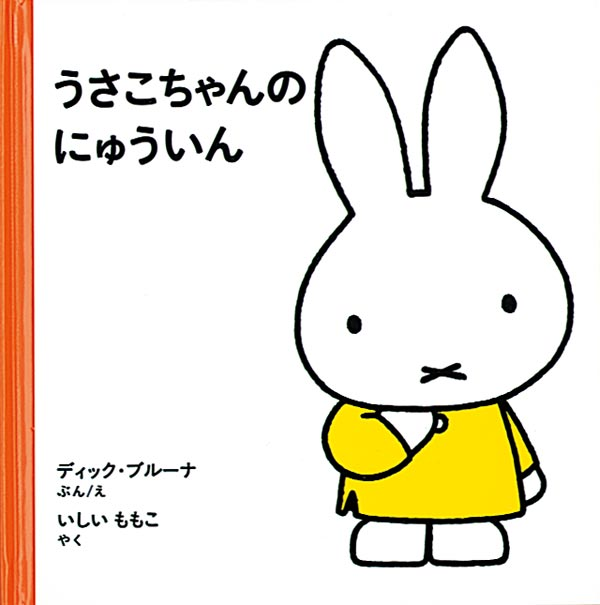
\includegraphics[width=5cm]{img/image.png}
  \caption{1975年のミッフィー}
  \label{miffy_1975}
\end{figure}

この画像を見ると今のミッフィーに比べ耳が角ばっているように見える.
昔のミッフィーとキャシーではウサギのキャラクターとして特徴的な耳のキャラクターデザインに大きな違いがあると考える.

以上のことを踏まえるとキャシーはミッフィーの複製ないし翻案には当たらないと考えられる.
\newpage
\section{現在の著作権法は、近年のデジタル化/ネットワーク化が進んだ社会に対して必ずしも対応しきれておらず、
  ある面で情報の自由な流通を妨げる存在であるともいえる状況である。
  そこで、著作権法本来の目的である文化の発展をさらに促進するために、本学にて
  あなたが学んでいる情報技術を活用してどのような改善を図ることが出来るか、独自
  のアイディアを創出し、その内容を簡単に説明せよ。}
近年,急速に発展したデジタル化・ネットワーク化や生成系AIの台頭によって誰でも簡単にある程度の水準の作品を出力できるようになった.
中でもStable Diffusionを代表とするようなイラストを生成するAIは違法サイトにアップロードされた画像を教師データに使用していたり,
有名な絵師がTwitterなどのSNSに挙げた画像を無断でAIに学習されて絵柄を模倣される等といった被害が出ている.

この問題のだめなところは,AIを使う人間がAIを使っていると明記しないことで人間が描いた絵がAIが描いたイラストに埋もれてしまうことに加え,
絵柄が模倣されてしまうので絵師が所有していた創作的で表現されているという独自性が失われてしまうことにある.

この件を解決するためには,AIイラストと絵師が描いたイラストの棲み分けが大事であると考える.
この棲み分けがうまく行った例として絵と写真の関係を挙げる.

絵はもともと現実世界を写し取ることが主な役割としてあげられていた.
また,写真も現実世界を写し取るが,白黒であったり撮るための条件が厳しかったりなどで絵が写真にシェアを大きく奪われることはなかった.
しかし,カメラの性能が上がってきたことで現実をよりリアルに写し取れるようになった.
だが,絵もSNSなどの普及に伴って絵としての立場を残しつつ,写真も発展したことで,近年では写真と絵はそれぞれ独立したコンテンツとして確立している.

よって,私が学んでいる情報技術を活用することで人が描いたイラストとAIイラストを棲み分けさせることでそれぞれが独立したコンテンツとして確立できるのではないかと考える.

% 参考文献
\newpage
\begin{thebibliography}{99}
  \bibitem{task2}違法アップロードで逮捕リスクのある行為と罰則!視聴のみでも逮捕?\url{https://wakailaw.com/keiji/13003/}
  \bibitem{task3_1}著作物とは?定義・要件・種類・具体例などを分かりやすく解説!\url{https://keiyaku-watch.jp/media/hourei/chosakubutsu/}
  \bibitem{task3_2}同一性保持権 - Wikipedia\url{https://ja.wikipedia.org/wiki/同一性保持権}
  \bibitem{task3_3}写真の一部削除・文字追加が同一性保持権の侵害にあたるとされた事例\url{https://bengoshi-sakao.com/column/写真の一部削除・文字追加が同一性保持権の侵害/}
  \bibitem{R6}令和6年度著作権テキスト\url{https://www.bunka.go.jp/seisaku/chosakuken/textbook/index.html}
  \bibitem{task5_1}ミッフィー - Wikipedia\url{https://ja.wikipedia.org/wiki/ミッフィー}
  \bibitem{task5_2}ハローキティ - Wikipedia\url{https://ja.wikipedia.org/wiki/ハローキティ}
  \bibitem{miffy_1975_fig}うさこちゃんのにゅういん|福音館書店\url{https://www.fukuinkan.co.jp/book/?id=447}
\end{thebibliography}

\end{document}